\chapter{Analyse}\label{ch:analyse}
Im Folgendem wird der Einsatz von cloud native bei der DATEV e.G. analysiert.
Im Vergleich dazu, wird der aktuelle Bereitstellungsprozess für die Laufzeitumgebung, dem dazugehörigen Datenbanksystem und einer Messaging Lösung erläutert.
Anschließend erfolgt eine Beschreibung der Beispielanwendung \glqq DATEV-Rechnungsschreibung\grqq.
Die dafür benötigten Informationen stammen aus Gesprächen mit Mitarbeiter 1 aus der Abteilung, die für die DATEV-Rechnungsschreibung zuständig ist.
Es wird vor allem der technische Aspekt beleuchtet.

\section{Analyse von cloud native bei DATEV e.G.}\label{sec:analysecloud}
Neben den im Absatz \ref{sec:cloudnative} beschriebenen Begriffe, \glqq cloud native\grqq, \glqq Cloud Foundry\grqq{} und \glqq CI/CD\grqq{} ist der sogenannte \glqq DevOps\grqq-Gedanke in diesem Zusammenhang bei der DATEV e.G. von Bedeutung.
Laut dem Buch \glqq The Phoenix Project\grqq{} von Gene Kim\footnote{\cite{Kim.2014}} lassen sich die Werte und die Philosophie von DevOps in \glqq Three Ways\grqq{} erläutern.

\paragraph{\glqq The First Way\grqq} betrachtet den Fluss von der Entwicklung über die Middleware Verwaltung bis hin zum Kunden.
Um diesen Fluss zu optimieren, sollten möglichst kleine Änderungen in möglichst kleinen Arbeitsabschnitten entwickelt werden.
Dabei helfen unter anderem Continuous Integration\footnote{Siehe Absatz \ref{sec:cicd}}, Continuous Delivery\footnote{Siehe Absatz \ref{sec:cicd}} und das automatische Erstellen von Laufzeitumgebungen nach Bedarf.

\paragraph{\glqq The Second Way\grqq} betrachtet den Feedback-Fluss über alle Stages hinweg.
Ziel dabei ist, möglichst schnell Fehler zu erkennen und diese zu beheben oder gar zu vermeiden.
Zur Erreichung dieses Ziels gehört unter anderem das Abschaffen der sog. \glqq Schubladendenkweise\grqq.
Ein Beispiel aus Entwicklersicht:\\
\glqq Meine Anwendung läuft nicht... Ach da gibt es Probleme mit dem Webserver, dass werden die Kollegen der Administration schon lösen\grqq.

\paragraph{\glqq The Third Way\grqq} betrachtet weniger den Prozess an sich, sondern eher das Schaffen einer Kultur.
Eine Kultur, die erlaubt Risiken einzugehen und aus Fehlern zu lernen, aber auch das Verständnis, dass Wiederholung und Übung Voraussetzung für einen guten Entwickler sind.
Dabei ist ein hoher Grad an Vertrauen in das Team notwendig.

Bei der DATEV e.G. wird dieser DevOps-Gedanke durch sogenannte \glqq Product-Teams\grqq umgesetzt.
In einem solchen Team kümmert man sich neben der eigentlichen Softwareentwicklung, Testmaßnahmen usw. auch um den Betrieb der Middleware, z.B. die im Cloud Native Umfeld üblichen noSQL Datenbanken wie Mongo oder PostgreSQL. 
Dem ganzen Team wird viel Vertrauen gegeben und es soll weitestgehend autonom Software erstellen und betreiben können.
Dadurch steigt die Effektivität des Teams.

Die Kombination mit einer automatisierten CI/CD-Pipeline birgt weitere Vorteile.
So sorgt Continuous Integration dafür, dass individuelle Codeänderungen sofort nach der Integration in die Codebasis auf Korrektheit geprüft werden.
Im Fehlerfall werden die Entwickler sofort automatisch benachrichtigt. 
Verbunden mit regelmäßiger Integration führt das zu einer schnelleren und einfacheren Fehlerbehebung.
Ein weiterer Vorteil ist, dass neben der Prüfung auf Korrektheit auch eine statische Codeanalyse möglich ist.
Dadurch kann sichergestellt werden, dass der Code den gewünschten Qualitätskriterien entspricht.
Durch Continuous Delivery und Continuous Deployment kommen diese Änderungen im Idealfall voll automatisiert beim Kunden an.
Auch dies führt  zu einer Effizienzsteigerung.

Für die Bereitstellung der benötigten Laufzeitumgebung kommt bei DATEV e.G. die Cloud Foundry Distribution von \glqq pivotal\grqq{} als PaaS Plattform zum Einsatz.
Durch den darin zur Verfügung gestellten \glqq Marketplace\grqq{} können Laufzeitumgebungen effizient \glqq auf Knopfdruck\grqq generiert werden.
Mittels des Kommandozeileninterfaces kann die Bereitstellung auch in eine CI/CD-Pipeline integriert werden.
So werden z.B. für jeden Entwickler isolierte Testumgebungen geschaffen.

\section{Aktueller Bereitstellungsprozess}\label{sec:aktbereit}
Im Vergleich zu den Product-Teams im cloud native Umfeld, bei denen sich das Team selbst um den Betrieb der Middleware kümmert, verwalten im z/OS Umfeld eigens dafür zuständige Administratorenteams die Middleware auf allen Stages.
Die \glqq CICS Administration\grqq{} kümmert sich um alles rund um das CICS Subsystem.
Die \glqq Db2 Administration\grqq{} stellt Datenbanken und Tabellen auf Anfrage der Entwickler bereit.
Die \glqq IBM MQ Administration\grqq{} verwaltet die IBM MQ Ressourcen.
Um die Bereiche, an denen das \glqq IBM Cloud Provisioning and Management for z/OS\grqq-Tool helfen kann, identifizieren zu können, wird im Folgenden der aktuell etablierte Prozess für z/OS Anwendungen beschrieben.
Die in diesem Absatz genannten Informationen stammen aus Gesprächen mit Mitarbeitern aus den jeweiligen Administratorenteams.
Wie in Absatz \ref{sec:zosanw} beschrieben benötigt eine z/OS Anwendung zunächst eine Laufzeitumgebung, im Fall dieser Arbeit handelt es sich um CICS.

\subsection{Bereitstellung einer CICS Instanz}\label{ssec:aktcics}
Um eine lauffähige CICS-Instanz einzurichten, sind mehrere Schritte notwendig.
Der komplette Prozess wird in Abbildung \ref{fig:aktcics} dargestellt.
Wie zu sehen ist, ist der Initiator des Prozesses das Entwicklerteam.
Zunächst wird dort während der Entwicklungsphase festgestellt, dass ein neue CICS-Instanz benötigt wird, z.B. um eine neue Fachlichkeit testen zu können. 
Hier hilft das CICS Administratorenteam mittels Beratung.
Während einer Beratungsphase, die via Telefon, Emails oder Terminen stattfindet, wird sichergestellt, ob wirklich eine neue CICS-Instanz notwendig ist oder ob nicht eine bereits bestehende Instanz genutzt werden kann, die dann aber meist wieder zwischen Anwendungen und Entwicklern geteilt wird.
Falls eine neue CICS-Instanz benötigt wird, wird ein \Gls{racf} Eintrag für diese Instanz beantragt.
Dieser Eintrag wird dann vom RACF Team erzeugt.
Um sicherzustellen, dass die CICS-Instanz in den täglichen Sicherungen enthalten ist, muss das System Automations-Team benachrichtigt werden.

\begin{figure}[ht!]
\centering
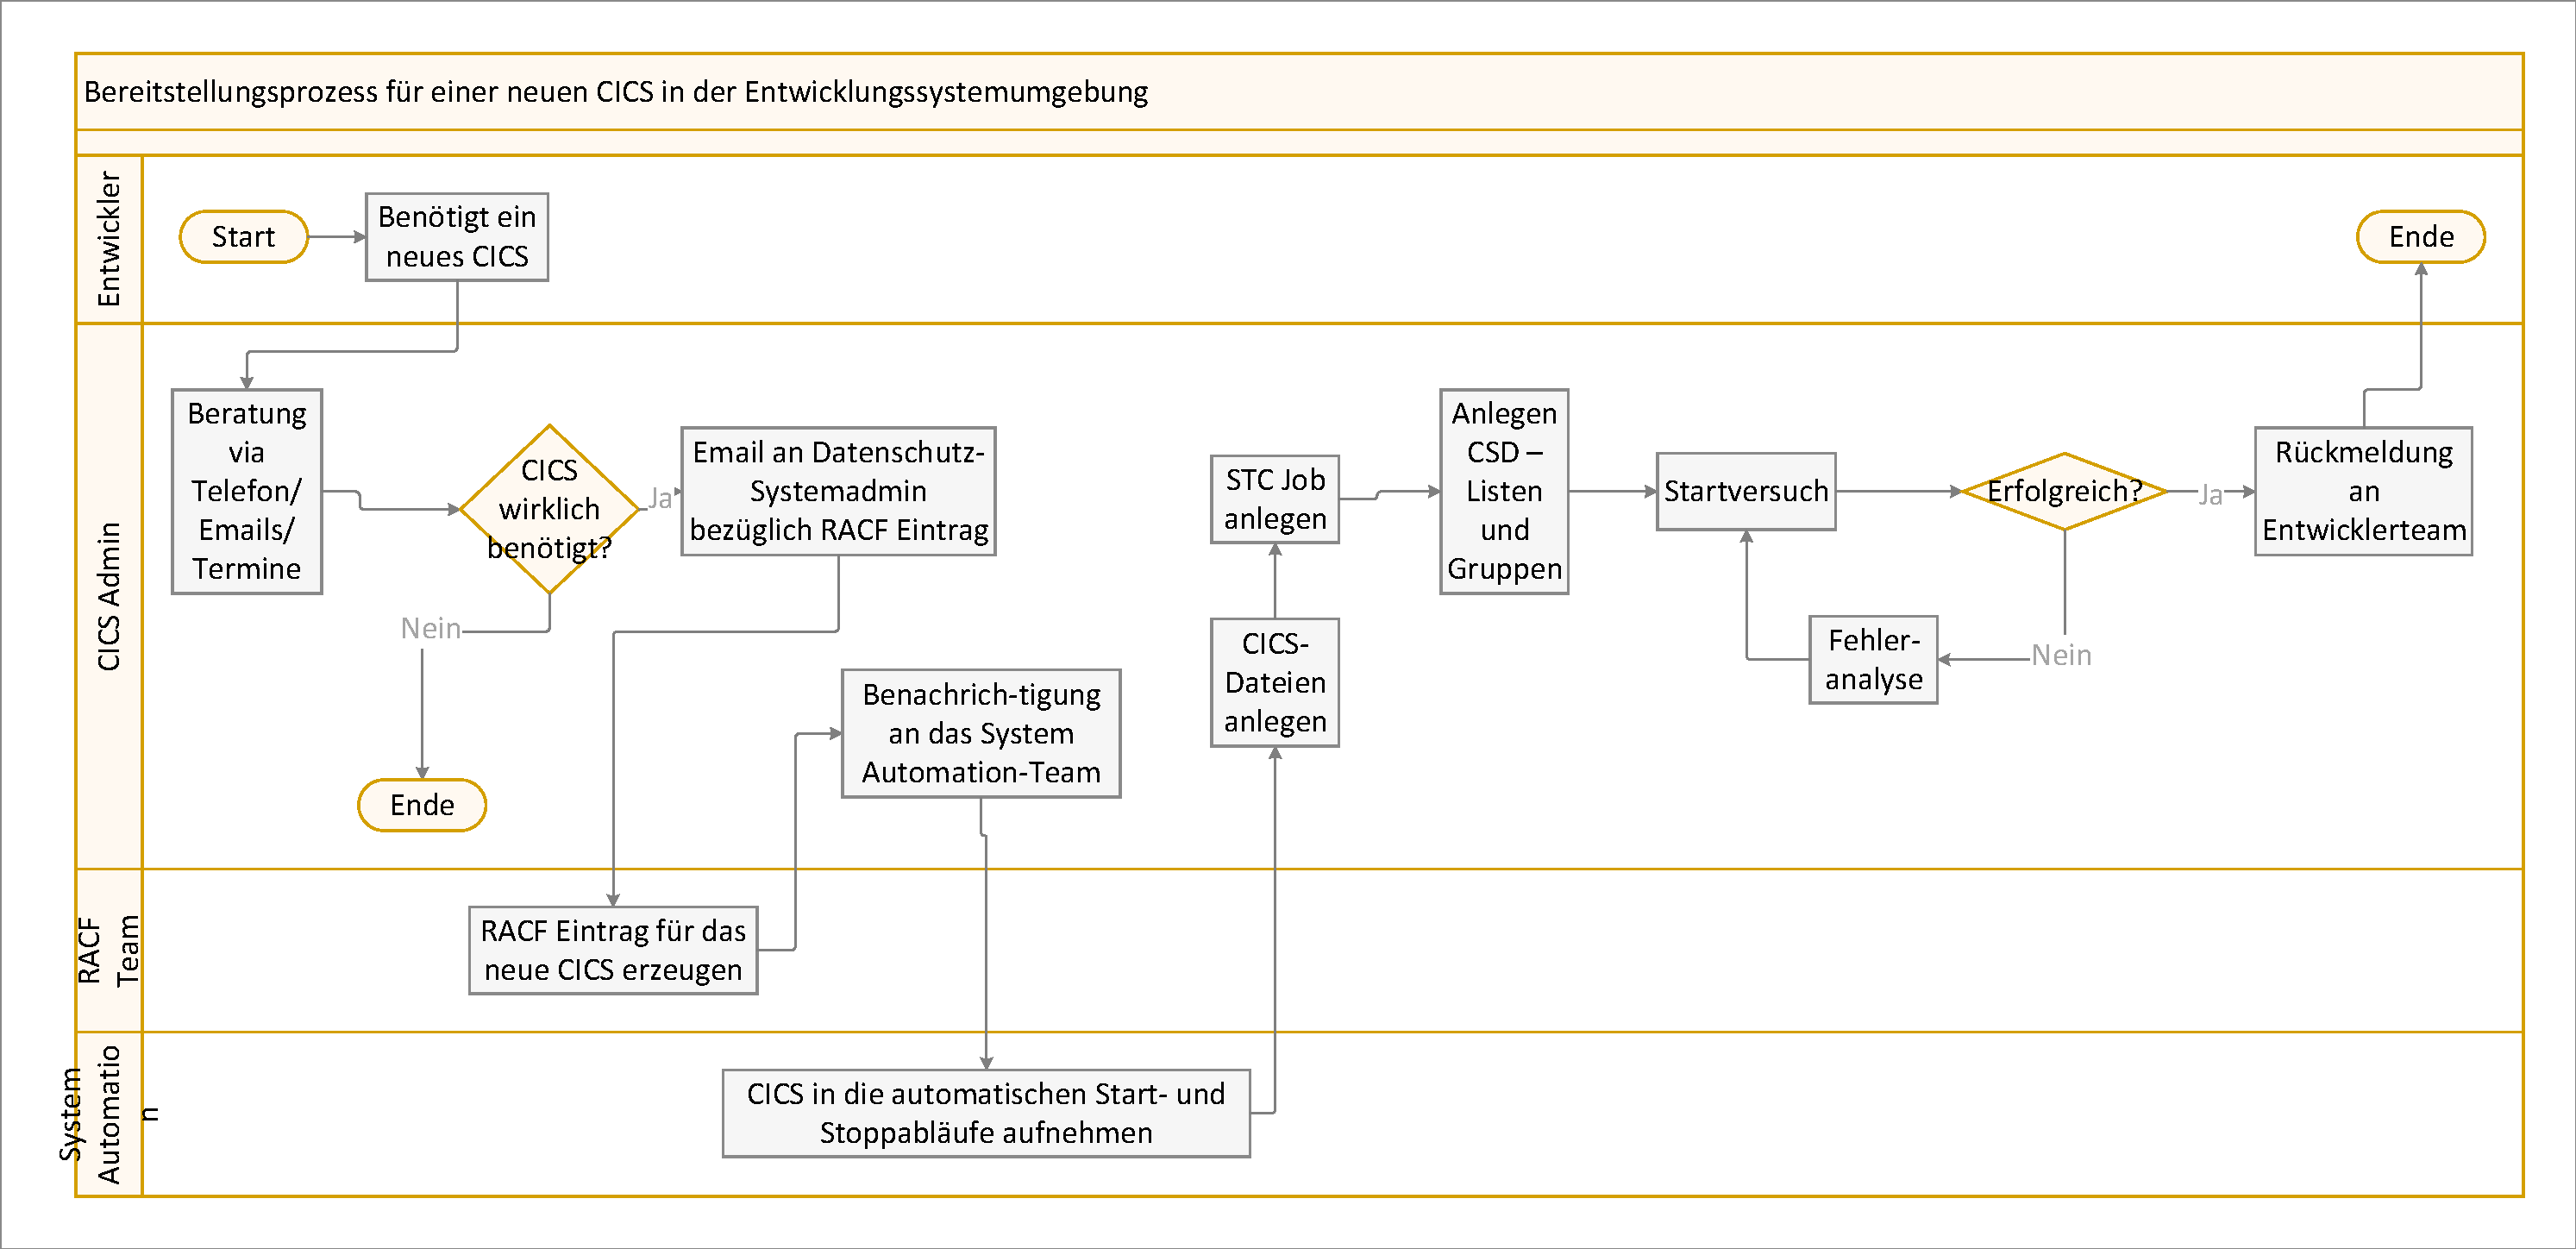
\includegraphics[width=\paperwidth,angle=90]{figures/swimlaneCICS.pdf}
\caption{Bereitstellungsprozess einer CICS Instanz}
\label{fig:aktcics}
\end{figure}

Nun kann mit dem eigentlichen Anlegen der CICS-Instanz begonnen werdem.
Dabei müssen folgende Schritte manuell durchgeführt werden.
Es werden nur die Schritte, die im Laufe dieser Arbeit durch das \glqq IBM Cloud Provisioning and Management for z/OS\grqq-Toolkit automatisiert werden, dargestellt.
Es handelt sich um das Anlegen von:

\begin{itemize}
\item CICS spezifische Dateien
\item \glqq CICS System Definition\grqq
\item Started Task Control-Job
\end{itemize}

\paragraph{CICS spezifische Dateien}\label{sssec:speziDat} ~\\
Zunächst müssen CICS spezifische Dateien im z/OS angelegt werden.
Im Fall des dieser Arbeit zugrunde liegenden Beispiels handelt es sich um siebzehn verschiedene VSAM Dateien.
Diese Dateien benötigt die CICS-Instanz um zum Beispiel Systemfehler zu protokollieren oder den Debugger aktivieren zu können.

\paragraph{\glqq CICS System Definition\grqq} ~\\
In der Datei \glqq CICS System Definition\grqq, kurz CSD, muss jede Ressource, die dem System zur Verfügung stehen soll, definiert werden.
Eine CSD Datei kann für mehrere CICS-Instanzen verwendet werden und besteht aus mehreren Einträgen.
Ein Eintrag besteht aus einer Gruppe und einer Liste.
Die Gruppe ist hierbei die Definition einer Systemressource und muss manuell angelegt werden.
Bei der Liste handelt es sich um das System, welches diese Ressource benötigt.
Dort ist unter anderem für jede CICS-Instanz hinterlegt, zu welchem Db2 Datenbankmanagementsystem und welchem MQ Queue Manager sich diese Instanz verbinden soll.
Somit können Transaktionen auf diese beiden Ressourcen zugreifen.

\paragraph{Started Task Control-Job} ~\\
Bei einem Started Task Control-Job, kurz STC Job, handelt es sich um einen langlaufenden Batch Job, der mit Hilfe des \glqq START\grqq-Konsolenkommandos innerhalb von z/OS gestartet werden kann.
Dieser Batch Job wird deshalb auch als Started Task bezeichnet.\cite{Cassier.2007}
Bei der DATEV e.G. existiert für jede Instanz eines Subsystems (z.B. CICS) ein solcher Job.
In diesem werden zunächst einige zur Laufzeit benötigten Bibliotheken und Dateien eingebunden, unter anderem die CICS spezifischen Dateien\footnote{Beschreibung in Absatz \ref{sssec:speziDat}}.
Außerdem werden hier die SIT \footnote{CICS system initialization table} Parameter definiert.
Zunächst wird festgelegt welche Standard SIT verwendet werden soll.
Anschließend können diese Standardwerte überschrieben werden.
Zu diesen Parametern zählen unter anderem der eindeutige Name der CICS-Instanz, der Speicherort der dazugehörenden CSD und die Information, ob eine Verbindung zu einem Db2 Datenbankmanagementsystem und/oder zu einem Queue Manager hergestellt werden soll.

Nach der Durchführung dieser Schritte wird das CICS gestartet und es steht dem Entwickler eine neue CICS-Instanz zur Verfügung.
Der komplette Ablauf dauert, unter der Annahme, dass alle Beteiligten verfügbar sind, nur diese Anforderung umsetzen müssen und für die Beratung ein Arbeitstag veranschlagt wird, circa zwei Arbeitstage.

\subsection{Bereitstellungsprozess einer Db2 Datenbank}
Wie in Abbildung \ref{fig:aktdb2} zu erkennen ist, ist der Bereitstellungsprozess einer neuen Db2 Datenbank mit vielen Aufgaben im Entwicklerteam verbunden.
\begin{figure}[ht!]
\centering
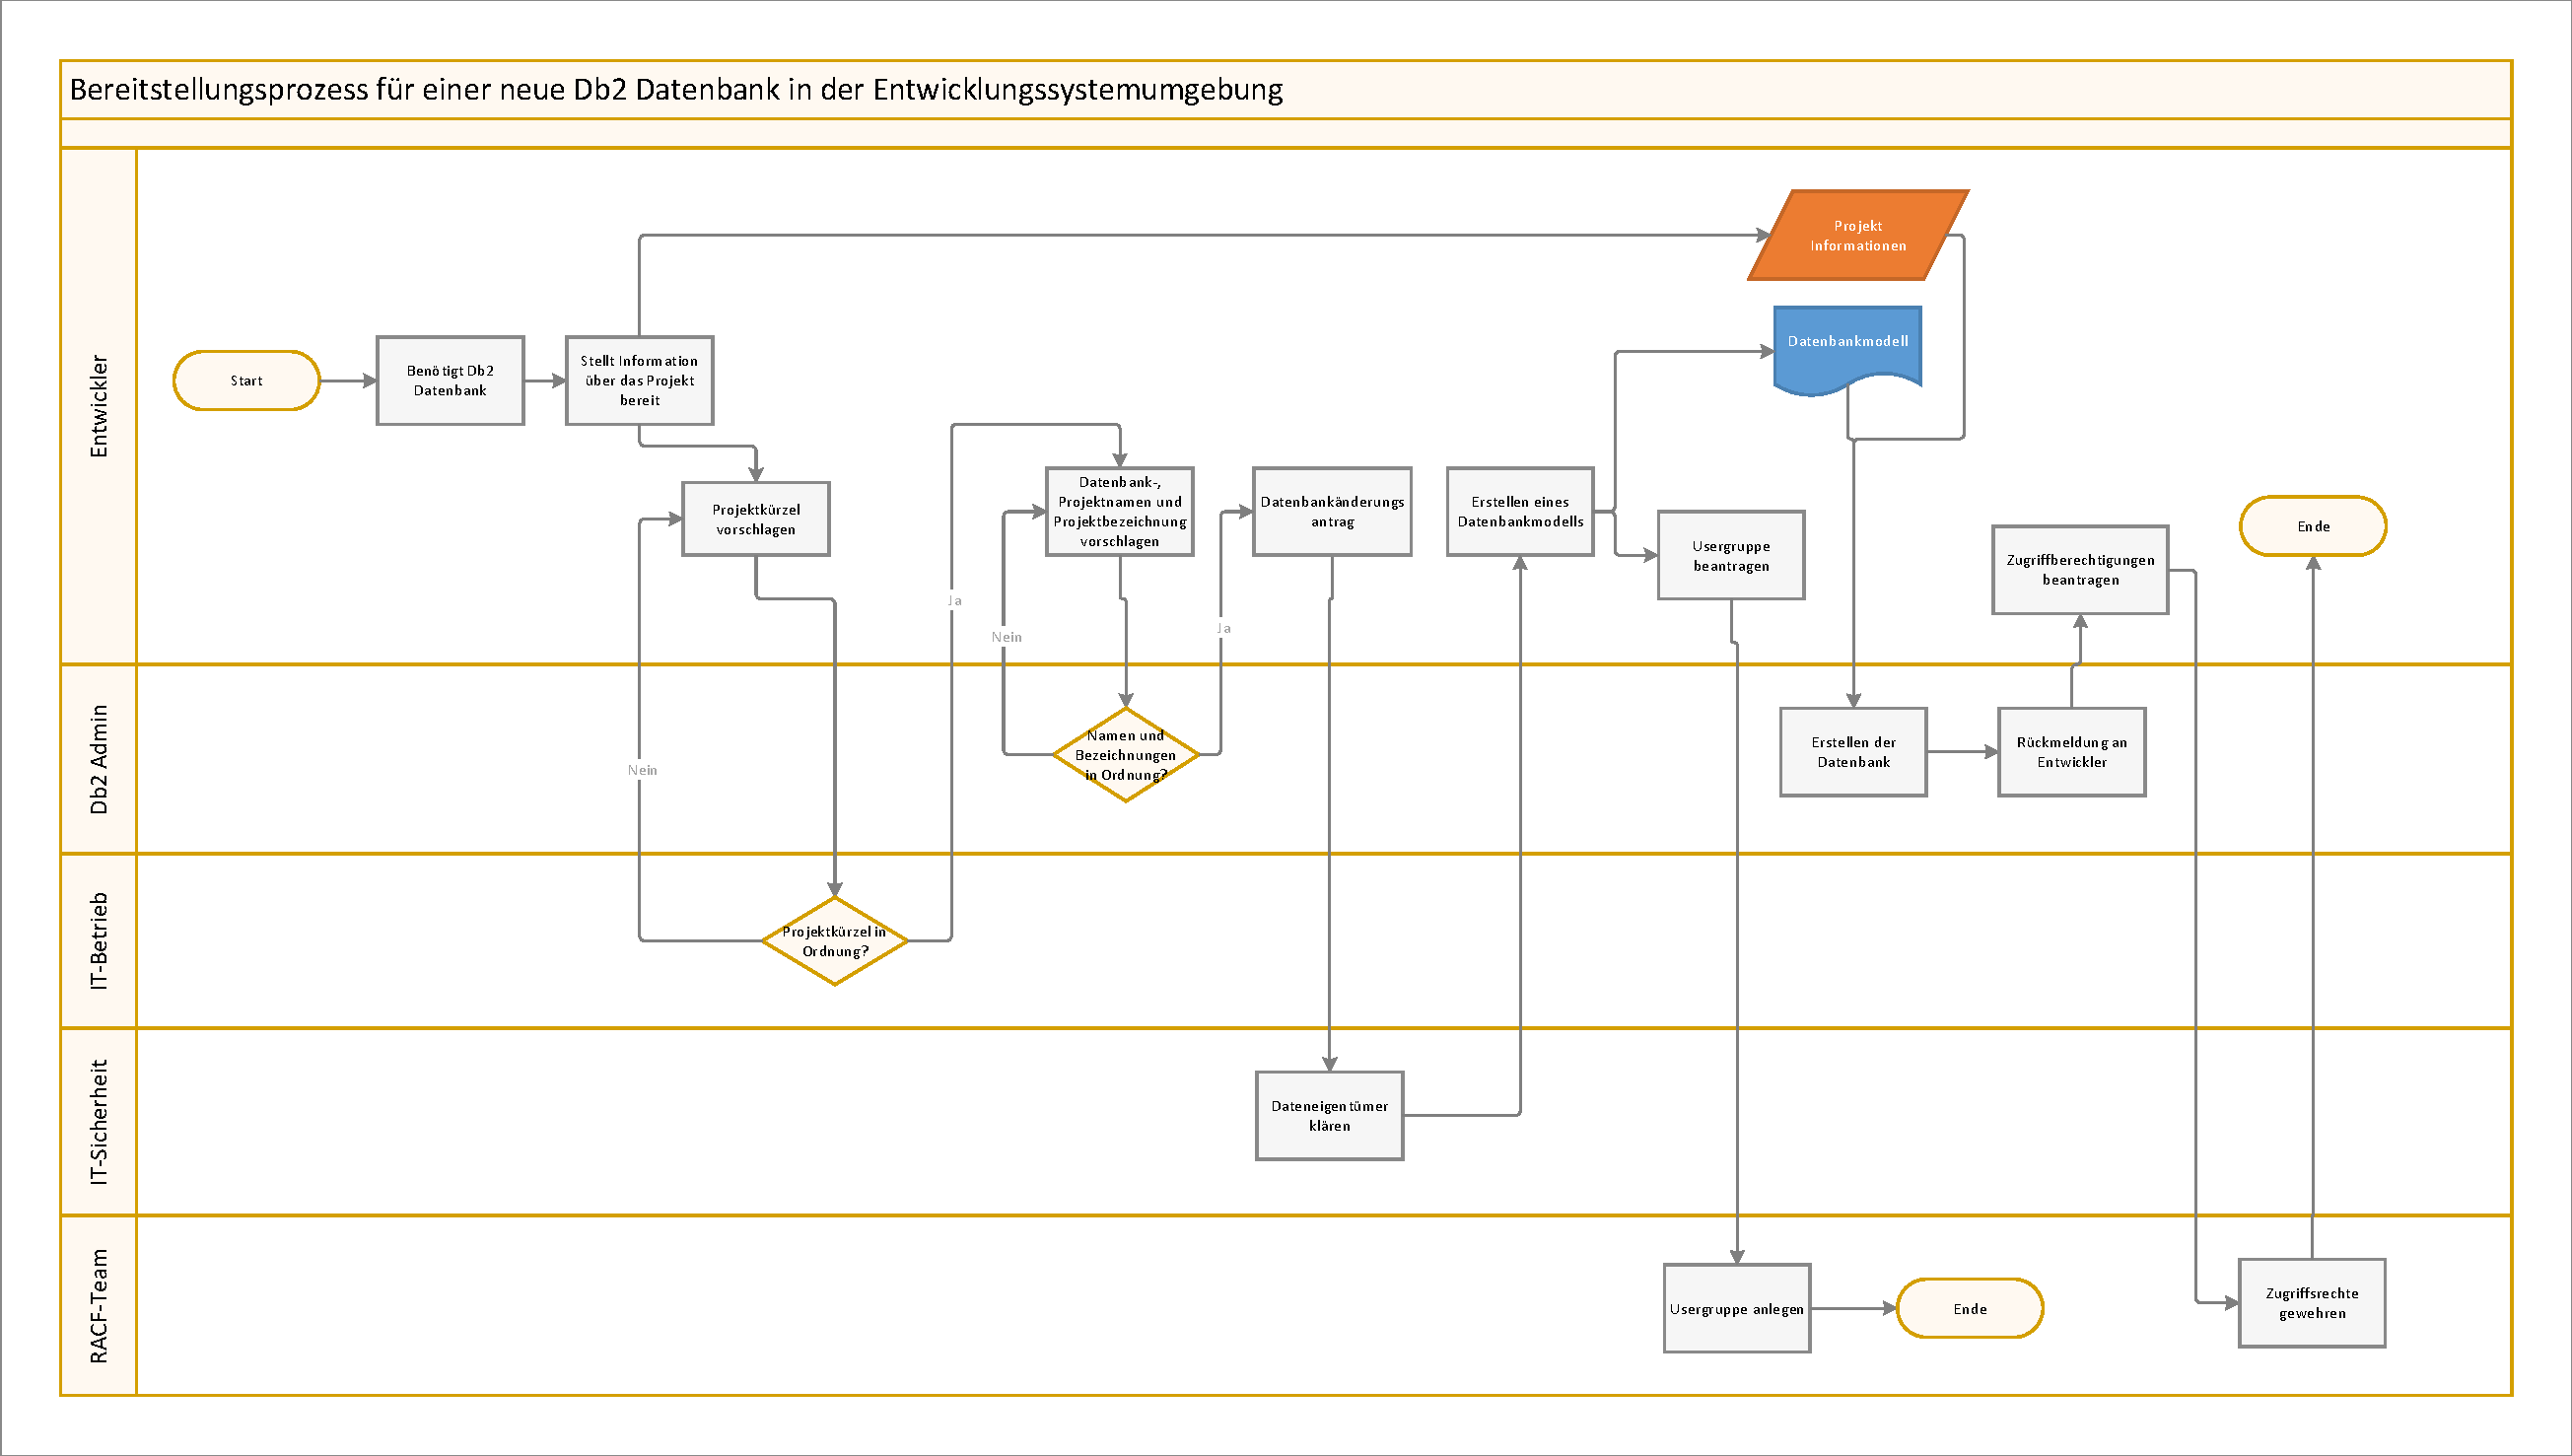
\includegraphics[width=\paperwidth,angle=90]{figures/swimlaneDb2.pdf}
\caption{Bereistellungsprozess einer Db2 Datenbank}
\label{fig:aktdb2}
\end{figure}
Zunächst müssen sogenannte Projektinformationen, unter anderem Daten der Voruntersuchung, vom Entwicklerteam bereitgestellt werden.
Das Projektkürzel\footnote{eindeutige Kennung von DATEV Projekten}, der Datenbank- und Projektname und die Projektbezeichnung müssen mit den involvierten Abteilungen besprochen werden.
Über den sogenannten \glqq Datenbankänderungsantrag\grqq{} wird ein Genehmigungsprozess angestoßen.
Wenn alle Genehmigungen erteilt wurden, kann ein Dateneigentümer festgelegt werden.
Anschließend muss die Datenbank mittels eines Datenbankmodells vom Entwicklerteam beschrieben werden und eine Usergruppe, die im späteren Verlauf die Datenbankzugriffsrechte benötigt, beantragt und angelegt werden.
Die eigentliche manuelle Erstellung der Datenbank wird mittels des Datenbankmodells und den Projektinformationen im Anschluss dazu durchgeführt.

Die Zugriffsrechte für die zuvor angeforderte Usergruppe auf die neue Datenbank werden beantragt.
Schließlich steht dem Entwicklerteam die neue Db2 Datenbank zur Verfügung.
Wird die Db2 Datenbank in Verbindung mit einem CICS verwendet, wie im Fallbeispiel dieser Arbeit, der DATEV-Rechnungsschreibung, so muss der entsprechende Eintrag in die CSD Datei manuell aufgenommen werden. 
Der komplette Ablauf dauert, unter der Annahme, dass alle Beteiligten verfügbar sind, nur diese Anforderung umsetzen müssen und für die Beratung ein Arbeitstag veranschlagt wird, circa zwei Arbeitstage.

\subsection{Bereitstellungsprozess einer IBM MQ Queue}
Auch bei dem Bereitstellungsprozess, siehe Abbildung \ref{fig:aktmq}, einer IBM MQ Queue ist das Entwicklerteam der Initiator.

\begin{figure}[ht!]
\centering
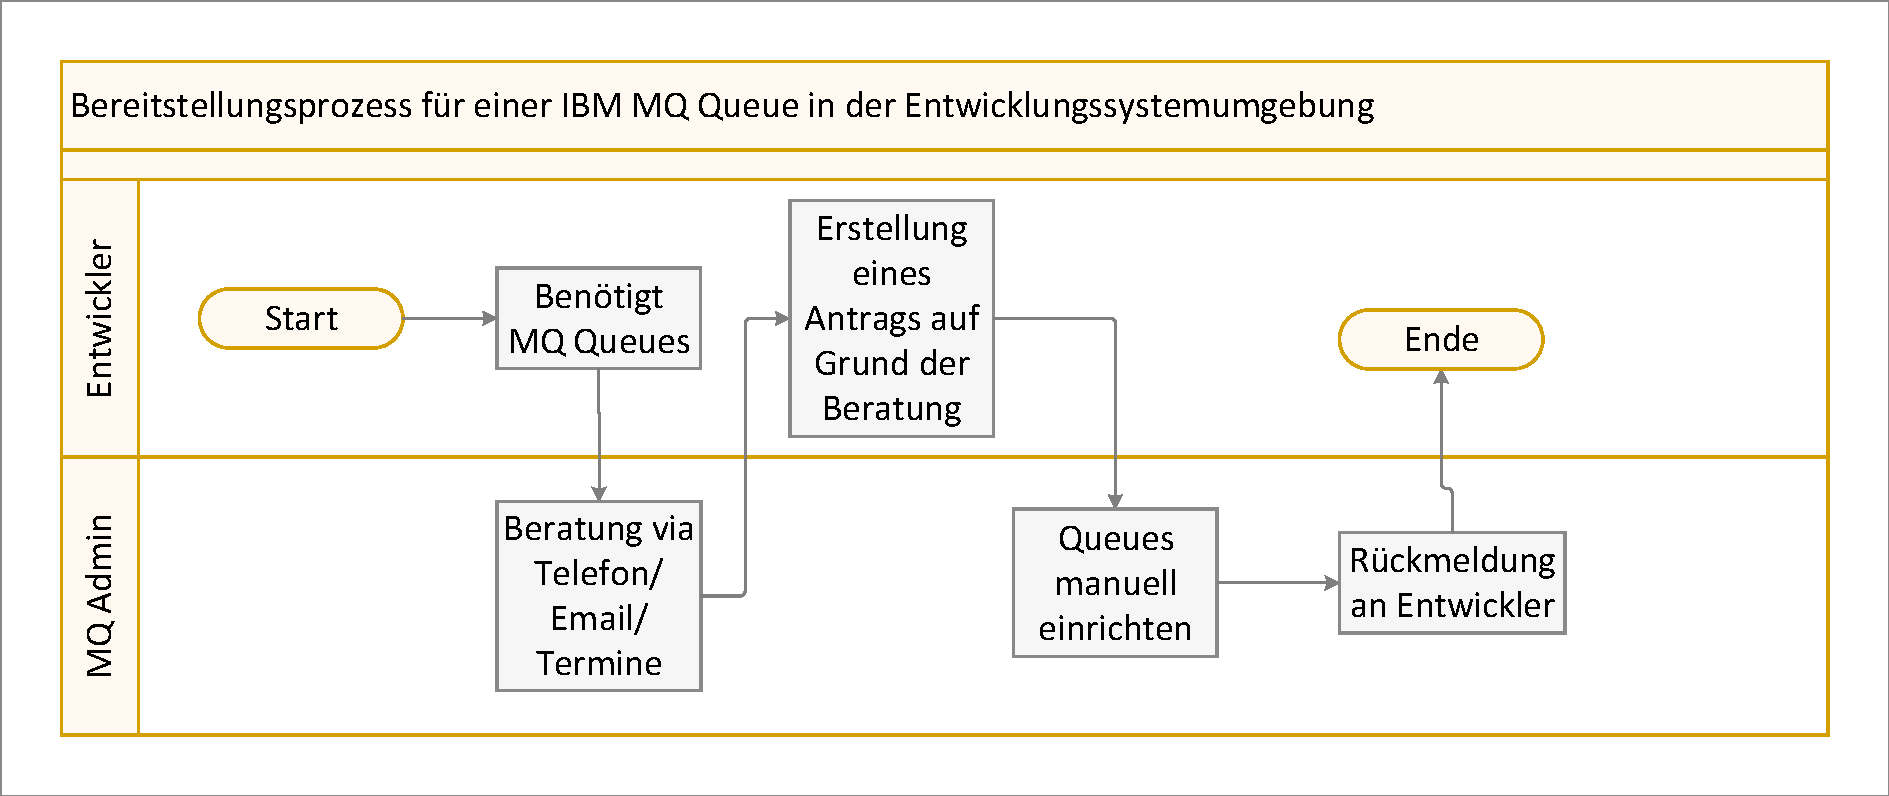
\includegraphics[width=\paperwidth,angle=90]{figures/swimlaneMQ.pdf}
\caption{Bereistellungsprozess einer IBM MQ Queue}
\label{fig:aktmq}
\end{figure}

Die Grundlage diese Prozesses ist ein Antrag auf Erstellung einer neuen IBM MQ Queue.
Zuvor findet eine Beratung via Telefon, Email oder Terminen statt.
Die Queues werden anschließend manuell eingerichtet und stehen dem Entwicklerteam zur Verfügung.
Wird die Queue in Verbindung mit einem CICS verwendet, so muss der Queue Manger auf dem die Queue angelegt wurde dem CICS mittels einem entsprechenden Eintrag in die CSD Datei mitgeteilt werden.
Trotz des scheinbar schmalen Prozesses dauert der Ablauf unter der Annahme, dass alle Beteiligten verfügbar sind, sie nur diese Anforderung umsetzen müssen und für die Beratung ein Arbeitstag veranschlagt wird, circa zwei Arbeitstage.

\subsection{Zusammenfassung aktueller Bereitstellungsprozess}\label{ssec:sumaktbereit}
Wie in den drei Diagrammen, Abbildungen \ref{fig:aktcics}, \ref{fig:aktdb2} und \ref{fig:aktmq}, zu erkennen ist, ist der aktuelle Bereitstellungsprozess mit vielen manuellen Schritten verbunden.
Der Hauptaufwand liegt bei den Administratorenteams, die in verschiedenen organisatorischen Einheiten angesiedelt sind.
Das Entwicklerteam ist  Initiator des Ablaufs.
Folglich kümmert es sich um die erforderlichen Formulare und die erste Kontaktaufnahme zum jeweiligen Administratorenteam.

Zusätzlich zu den zahlreichen manuellen Schritten sind die vielen Absprachen zwischen mehreren Abteilungen zu nennen.
Steht ein beteiligtes Team nicht zu Verfügung, oder sind andere Projekte höher priorisiert, kommt es zu Verzögerungen, das Entwicklungsteam muss warten, der komplette Zeitplan kann sich dadurch nach hinten verschieben.
Der Prozess für die Bereitstellung einer neuen CICS-Instanz, mit einer Db2 Datenbank und IBM MQ Queues dauert in der Summe circa sechs Arbeitstage.
Es setzt sich aus der Dauer der Einzelprozesse zusammen, für jedes Subsystem wird mit circa zwei Arbeitstagen gerechnet.
Natürlich ist ein parallelisierter Ablauf der einzelnen Teilprozesse möglich, so kann die Gesamtdauer im besten Fall auf circa zwei bis drei Arbeitstage verkürzt werden. 

Der Start des gesamten Prozesses findet meist auf \glqq Zuruf\grqq{} statt.
So existiert für die erste Kontaktaufnahme kein Formular, keine Automation oder ähnliches.
Es wird auf E-Mail, Telefon oder mittels Terminen zurückgegriffen.

Wird jetzt der Vergleich zu dem Bereitstellungsprozess im cloud native-Umfeld\footnote{Siehe Absatz \ref{sec:analysecloud}} in folgenden Punkten gezogen, so steht dem automatisierten und dadurch effizienten cloud native Prozess, ein durch viele Absprachen langsamer und fehleranfälliger Prozess auf z/OS gegenüber.

\begin{itemize}
\item Produktautonomie
\item Deployment
\item Architektur
\end{itemize}

\paragraph{Produktautonomie}~\\
Die Autonomie eines Product-Teams ist hier nicht gegeben, die Administratorenteams sind für den Betrieb der Subsysteme verantwortlich.
Daran wird sich auch durch automatisierte Provisionierung in Zukunft nichts ändern, da hier hohes Spezialistenwissen benötigt wird, das nicht von jedem Product-Team bereitgestellt werden kann. 
Dazu kommt, dass die Provisionierung im Rahmen dieser Arbeit auch nur die Bereitstellung von Entwicklungs-Instanzen der Middleware Systeme betrachtet. 
Die Administratorenteams sind aber insbesondere für die produktiven Instanzen im Betrieb verantwortlich, die nach wie vor von Anwendungen geteilt werden.  
D.h. der Cloud-Aspekt des automatischen Deployments einer Anwendung inklusive Runtime zwischen Stages wird also nicht umgesetzt.

\paragraph{Deployment}~\\
Da für das Deployment einer z/OS CICS Anwendung, wie in Absatz \ref{sssec:cicsanwd} beschrieben, Bibliotheken zum Einsatz kommen, muss beim Testen einer Anwendung immer geprüft werden, ob der aktuellste Stand der Anwendung in dieser Bibliothek abgelegt ist, ob die Bibliothek überhaupt der CICS Instanz zur Verfügung steht und ob nicht eine andere Bibliothek mit anderem Stand von der CICS Instanz angezogen wird.
Diese Probleme verschlechtern sich, wenn an der gleichen Anwendung mehrere Mitarbeiter entwickeln, so ist viel Absprache notwendig, um beispielsweise nicht den Stand eines Kollegen zu überschreiben.

\paragraph{Architektur}~\\
Neben den Problemen im Bereitstellungsprozess ist die grundlegende Architektur einer z/OS Anwendung zu betrachten.
Im Vergleich zur \glqq Microservices\grqq-Architektur, die im cloud native Umfeld häufig zum Einsatz kommt\footnote{Siehe Absatz \ref{sec:cloudnative}}, sind klassische z/OS Anwendungen monolithisch aufgebaut.
Insbesondere aus Performancegründen, haben sich über die Jahre Abhängigkeiten und Verzahnungen zwischen einzelnen Anwendungen gebildet.
Diese starke Koppelung erhöht die Komplexität und erschwert das Testen dieser Anwendungen.

Wird der Architekturaspekt der geteilten Subsystem Ressourcen betrachtet, kristallisiert sich ein weiteres Problem heraus.
Es ist möglich, dass eine Anwendung eine komplette CICS Instanz zum Absturz bringt.
Ist dies der Fall sind auf Grund einer Anwendung alle anderen Anwendungen dieser CICS Instanz nicht mehr verfügbar.
Mit Hilfe von isolierten Testumgebungen kann dieser Problem gelöst werden.

Nach diesem Vergleich sieht die DATEV e.G. bei dem hier untersuchten automatisierten Prozess vor allem bei der Entwicklungseffizienz einen Vorteil.
Dabei wird der Fokus auf die Effizienz bei der Bereitstellung isolierter Testumgebungen, ohne Wartezeit und mit möglichst wenig manueller Interaktion gelegt.
Dadurch verspricht sich die DATEV e.G. kürzere Entwicklungszyklen und weniger Fehleranfälligkeit durch zu hohen Abstimmungsaufwand.


Hierzu wird in dieser Arbeit das Tool \glqq IBM Cloud Provisioning and Management for z/OS\grqq{} für die automatisierte Bereitstellung von Laufzeitumgebungen für die Entwicklungsstage untersucht.
Als Beispielanwendung dient ein Teil der z/OS Anwendung \glqq DATEV-Rechnungsschreibung\grqq.

\section{DATEV-Rechnungsschreibung}\label{rechBesch}
Für diese Arbeit wurde die DATEV-Rechnungsschreibung als Beispielanwendung herangezogen, weil sie folgenden Anforderungen entspricht.
Es handelt sich zum einem um eine in sich abgeschlossene Anwendung, die nur zu Beginn des Prozesses von anderen Anwendungen abhängig ist.
Zum anderen benötigt die DATEV-Rechnungsschreibung ein CICS als Laufzeitumgebung, eine Db2-Datenbank und IBM MQ als Messaginglösung.
Somit kann ein umfangreicher Bereitstellungsmechanismus untersucht werden.

Bei dem Gesamtablauf handelt es sich um einen Batch-Ablauf auf dem Großrechner der DATEV e.G.
Dieser setzt sich aus folgenden Teilen zusammen:
\begin{itemize}
\item Sammeln von Berechnungssätze
\item Tägliche Bewertung
\item Rechnungsaufbereitung
\end{itemize}
Für die Beantwortung der Forschungsfragen ist nur ein Teil der \glqq Tägliche Bewertung\grqq relevant, die Preisermittlung.

\subsection{Tägliche Bewertung}\label{sssec:täglbew}
Dieser Ablauf läuft einmal täglich von Montag bis Freitag und ist für die Preisermittlung und Kundenzuordnung zuständig.
Zur Realisierung wurden die Programmiersprachen Assembler, COBOL und Java genutzt.
Am Ende dieses Ablaufes steht die ARUBA\footnote{Abrechnungs- und Umsatz-Basis}-Db2-Datenbank.
Dort werden die Berechnungsdaten der letzten 36 Monate aufbewahrt.
Dabei handelt es ich um insgesamt circa 3,8 Milliarden Datensätze von einer Gesamtgröße von circa 400 GB mit Indizes.
Diese Datensätze beinhalten alle Informationen für die endgültige Erzeugung der Rechnungen.

\subsection{Preisermittlung}\label{ssec:preis}
Die Preisermittlung ist für die Berechnung der Preise mit den dazugehörigen kundenindividuellen Abhängigkeiten, beispielsweise Rabatte, zuständig.
Die Eingabe beläuft sich an Lasttagen auf bis zu 180.000 Geschäftspartner.
Im DATEV e.G. Umfeld ist ein Geschäftspartner entweder eine Kanzlei oder ein einzelner Mandant.
Aufgrund dieser Last wird die Berechnung in CICS durchgeführt und in folgende zwei Teile zerlegt:
\begin{itemize}
\item Bereitstellen der Preisinformationen
\item Berechnung der Preise
\end{itemize}
\paragraph{Bereitstellen der Preisinformationen}~\\
Bevor die eigentliche Ermittlung der Preise stattfindet, werden zunächst die Preisinformationen und die kundenindividuellen Preisabhängigkeiten, wie zum Beispiel Rabatte, ermittelt.
Für die Verarbeitung werden zwei Queues verwendet.
Eine startet eine Transaktion im CICS, die andere wartet auf deren Antwort.
Innerhalb der Transaktion werden alle benötigten Preisinformationen und -abhängigkeiten mit Hilfe einer Db2 Datenbank ermittelt.
Diese Informationen werden dann in einem sogenannten \glqq SHARED GETMAIN\grqq-Bereich gespeichert.
Dabei handelt es sich im Prinzip um einen Hauptspeicherbereich, der dem CICS Subsystem zur Verfügung steht.
Die Adresse dieses Bereiches wird den Transaktionen zur Verfügung gestellt.
Somit greifen die einzelnen Transaktionen nicht mehr direkt auf die Datenbank zu, sondern stattdessen auf den schnelleren Hauptspeicher.
Diese Vorarbeit ist notwendig, da die notwendige Performance aufgrund von bis zu 60 Millionen Datenbankzugriffen nicht erreicht werden würde.

\paragraph{Berechnung der Preise}~\\
Um die Berechnungsdaten der 180.000 Geschäftspartner an CICS-Instanzen zu übertragen, stehen dem System weitere Queues zur Verfügung.
Darunter ist eine allgemeine Queue, in der alle Aufträge, die für die Weiterverarbeitung zur Verfügung stehen, geschrieben werden.
Pro Geschäftspartner wird ein Auftrag angelegt.
In diesem Auftrag befinden sich die Namen vier weiterer Queues.
Eine dieser Queues beinhaltet alle Informationen, die für die Preisermittlung des dazugehörigen Geschäftspartners notwendig sind.
Hierzu zählt unter anderem die Adresse des vorher beschriebenen Hauptspeicherbereichs.
In den restlichen drei Queues sind die Ergebnisse der Preisermittlung gespeichert.
Die Ergebnisse stehen somit dem Batch-Ablauf zur Weiterverarbeitung zur Verfügung.
Für jede der vier Queues existieren jeweils 100 vorgefertigte Namen.
Somit können auch maximal nur 100 Aufträge gleichzeitig auf Weiterverarbeitung warten.
Falls dieses Limit erreicht ist, wartet der Batch-Ablauf so lange, bis einer der Aufträge fertig gestellt wird.
Sobald ein Auftrag in die allgemeinen Auftragsqueue geschrieben wird, wird eine CICS-Transaktion gestartet.
Diese führt die Preisermittlung durch und schreibt das Ergebnis auf die dazugehörigen Queues.
Ist dies geschehen, stehen die Queues wieder für einen neuen Auftrag zur Verfügung.
Es können maximal 30 Transaktionen zeitgleich arbeiten.
